\documentclass[a4paper]{article}

\usepackage[T1]{fontenc}
\usepackage[utf8]{inputenc}
\usepackage{mlmodern}

%\usepackage{ngerman}	% Sprachanpassung Deutsch

\usepackage{graphicx}
\usepackage{geometry}
\geometry{a4paper, top=15mm}

\usepackage{subcaption}
\usepackage[shortlabels]{enumitem}
\usepackage{amssymb}
\usepackage{amsthm}
\usepackage{amsmath}
\usepackage{mathtools}
\usepackage{braket}
\usepackage{bbm}
\usepackage{graphicx}
\usepackage{float}
\usepackage{yhmath}
\usepackage{tikz}
\usepackage{scratch}
\usetikzlibrary{patterns,decorations.pathmorphing,positioning}
\usetikzlibrary{calc,decorations.markings}

\usepackage[backend=biber, sorting=none]{biblatex}
\addbibresource{cite.bib}

\usepackage[framemethod=TikZ]{mdframed}

\tikzstyle{titlered} =
    [draw=black, thick, fill=white,%
        text=black, rectangle,
        right, minimum height=.7cm]


\usepackage[colorlinks=true,naturalnames=true,plainpages=false,pdfpagelabels=true]{hyperref}
\usepackage[parfill]{parskip}
\usepackage{lipsum}

\usepackage{tcolorbox}
\tcbuselibrary{skins,breakable}

\pagestyle{myheadings}

\colorlet{colexam}{black}
\newcounter{definition}
\newtcolorbox[use counter=definition]{mydef}[1]{
    empty,
    title={\textbf{Definition~\thetcbcounter}~~(\textit{#1})},
    attach boxed title to top left,
    fontupper=\sl,
    boxed title style={
        empty,
        size=minimal,
        bottomrule=1pt,
        top=1pt,
        left skip=0cm,
        overlay=
            {\draw[colexam,line width=1pt]([yshift=-0.4cm]frame.north
        west)--([yshift=-0.4cm]frame.north east);}},
            coltitle=colexam,
            fonttitle=\normalfont,
            before=\par\medskip\noindent,
            parbox=false,
            boxsep=-1pt,
            left=0.75cm,
            right=3mm,
            top=4pt,
            breakable,
            pad at break*=0mm,
            vfill before first,
            overlay unbroken={
                \draw[colexam,line width=1pt]
                ([xshift=0.6cm, yshift=-0.5pt]frame.south
                west)--([xshift=0.6cm,yshift=-1pt]frame.north west)
                --([xshift=0.6cm]frame.south west)--([xshift=-13cm]frame.south east); },
            overlay first={
                \draw[colexam,line width=1pt]
                ([xshift=0.6cm, yshift=-0.5pt]frame.south
                west)--([xshift=0.6cm,yshift=-1pt]frame.north west)
                --([xshift=0.6cm]frame.south west); },
            overlay last={
                \draw[colexam,line width=1pt]
                ([xshift=0.6cm, yshift=-0.5pt]frame.south
                west)--([xshift=0.6cm,yshift=-1pt]frame.north west)
                --([xshift=0.6cm]frame.south west)--([xshift=-13cm]frame.south east); }
}
\newcounter{theorem}
\newtcolorbox[use counter=theorem]{theorem}{
    empty,
    title={Theorem ~\thetcbcounter},
    attach boxed title to top left,
    fontupper=\sl,
    boxed title style={
        empty,
        size=minimal,
        bottomrule=1pt,
        top=1pt,
        left skip=0cm,
        overlay=
            {\draw[colexam,line width=1pt]([yshift=-0.4cm]frame.north
        west)--([yshift=-0.4cm]frame.north east);}},
            coltitle=colexam,
            fonttitle=\bfseries,
            before=\par\medskip\noindent,
            parbox=false,
            boxsep=-1pt,
            left=0.75cm,
            right=3mm,
            top=4pt,
            breakable,
            pad at break*=0mm,
            vfill before first,
            overlay unbroken={
                \draw[colexam,line width=1pt]
                ([xshift=0.6cm, yshift=-0.5pt]frame.south
                west)--([xshift=0.6cm,yshift=-1pt]frame.north west)
                --([xshift=0.6cm]frame.south west)--([xshift=-13cm]frame.south east); },
            overlay first={
                \draw[colexam,line width=1pt]
                ([xshift=0.6cm, yshift=-0.5pt]frame.south
                west)--([xshift=0.6cm,yshift=-1pt]frame.north west)
                --([xshift=0.6cm]frame.south west); },
            overlay last={
                \draw[colexam,line width=1pt]
                ([xshift=0.6cm, yshift=-0.5pt]frame.south
                west)--([xshift=0.6cm,yshift=-1pt]frame.north west)
                --([xshift=0.6cm]frame.south west)--([xshift=-13cm]frame.south east); }
}
\newcounter{lemma}
\newtcolorbox[use counter=lemma]{lemma}{
    empty,
    title={Lemma~\thetcbcounter},
    attach boxed title to top left,
    fontupper=\sl,
    boxed title style={
        empty,
        size=minimal,
        bottomrule=1pt,
        top=1pt,
        left skip=0cm,
        overlay=
            {\draw[colexam,line width=1pt]([yshift=-0.4cm]frame.north
        west)--([yshift=-0.4cm]frame.north east);}},
            coltitle=colexam,
            fonttitle=\bfseries,
            before=\par\medskip\noindent,
            parbox=false,
            boxsep=-1pt,
            left=0.75cm,
            right=3mm,
            top=4pt,
            breakable,
            pad at break*=0mm,
            vfill before first,
            overlay unbroken={
                \draw[colexam,line width=1pt]
                ([xshift=0.6cm, yshift=-0.5pt]frame.south
                west)--([xshift=0.6cm,yshift=-1pt]frame.north west)
                --([xshift=0.6cm]frame.south west)--([xshift=-13cm]frame.south east); },
            overlay first={
                \draw[colexam,line width=1pt]
                ([xshift=0.6cm, yshift=-0.5pt]frame.south
                west)--([xshift=0.6cm,yshift=-1pt]frame.north west)
                --([xshift=0.6cm]frame.south west); },
            overlay last={
                \draw[colexam,line width=1pt]
                ([xshift=0.6cm, yshift=-0.5pt]frame.south
                west)--([xshift=0.6cm,yshift=-1pt]frame.north west)
                --([xshift=0.6cm]frame.south west)--([xshift=-13cm]frame.south east); }
}

\newcommand{\eps}{\varepsilon}
\usepackage[OT2,T1]{fontenc}
\DeclareSymbolFont{cyrletters}{OT2}{wncyr}{m}{n}
\DeclareMathSymbol{\Sha}{\mathalpha}{cyrletters}{"58}

\markright{Popović\hfill Seminar\hfill}


\title{University of Vienna\\
\vspace{1cm}Seminar:\\Joint RICAM Seminar\\
\vspace{0.5cm}
Summary of talk by Otmar Scherzer
}
\author{Milutin Popovic}


\usepackage[final]{pdfpages}

\begin{document}
\maketitle
\tableofcontents
\section{Sheet 2}
\subsection{Problem 1}
\subsubsection{}
We let $\rho(A)$ be the spectral radius of a matrix $A \in
\mathbb{R}^{n\times n}$. A matrix norm $ \|\cdot\|_{1}$ is consistent with the
vector norm $\|\cdot\|_{2}$ if
\begin{align}
    \|Ax\|_{2} \le \|A\|_1\|x\|_2
\end{align}
for all $x \in \mathbb{R}^n$ and all $A \in \mathbb{R}^{n\times n}$. Indeed
every matrix norm induced by a vector norm is consistent. To show this let
$\|\cdot\|_M$ be a matrix norm and $\|\cdot\|_v$ be a vector norm, defined as
\begin{align}
    \|x\|_v = \|xv^T\|_M
\end{align}
for all $x \in \mathbb{R}^n$ and some $v \neq 0$, of $\mathbb{R}^{n \times
n}$ and $\mathbb{R}^{n}$ respectively. Then we have
\begin{align}
    \|Ax\|_v = \|Axv^T\| \le \|A\|_M \|xv^T\|_M = \|A\|_M \|v\|_v \qed
\end{align}
Note that for $\mathbb{C}^{n \times n}$ and $\mathbb{C}^{n}$ use $v^* \neq 0$ the
conjugate transpose.
\subsubsection{}
Now we consider a splitting of $A = D - (L + U)$, were $D, L$ and $U$ are
defined as
\begin{align}
    D &= \text{diag}\left(a_{11},\ldots,a_{nn}\right), \\
    \left(L \right)_{ij} &=
    \begin{cases}
        -\left( A \right)_{ij}\quad i > j\\
        0 \quad i\leq 0
    \end{cases},
    \qquad
    \left(U \right)_{ij} =
    \begin{cases}
        -\left( A \right)_{ij}\quad i < j\\
        0 \quad i \ge 0
    \end{cases},
\end{align}
Then the matrix of a single Jacobi iteration method is
\begin{align}
    B_J = D^{-1}(L+U)
\end{align}
We can show that if $A$ is strictly diagonally dominant then
\begin{align}
    \rho(B_J) \le \|B_J\|_\infty < 1.
\end{align}
If A is strictly diagonally dominant, this means that
\begin{align}
    &\mid A_{ii}\mid > \sum_{j\neq i}^{n}  \mid A_{ij} \mid \qquad \forall\
     i\in\{1, \ldots , n\} \\
    \Leftrightarrow &\sum_{j\neq i} \frac{ \mid A_{ij} \mid}{ \mid A_{ii}  \mid}
     < 1.
\end{align}
Now let $(\lambda, v)$ be an eigen-pair of $B_J$, then
\begin{align}
    B_J v &= D^{-1}(L+U)v = \lambda v\\
    (L+U)v &= \lambda D v.
\end{align}
For a chosen $i$ this means
\begin{align}
    \left| \lambda \right| \left| A_{ii} \right| \left| v_i \right|
    &=
    \left|
    -\sum_{j>i} A_{ij}v_i - \sum_{j<i} A_{ij}v_i
    \right|\\
    &\le \sum_{j>i}
    \left|A_{ij} \right| \left| v_i \right| + \sum_{j<i}
    \left|A_{ij} \right| \left| v_i \right|\\
    &= \sum_{j\neq i} \left| A_{ij} \right| \left|v_i\right|.
\end{align}
We can choose and $i$ such that $\left| v_i \right| \le \|v\|_\infty$, then
\begin{align}
    \left| \lambda \right| \left| A_{ii} \right| \left| v_i \right|
    &\le \sum_{j\neq i} \left| A_{ij} \right| \|v\|_\infty\\
    \Rightarrow
    \left| \lambda \right| \left| A_{ii} \right|
    &\le \sum_{j\neq i} \left| A_{ij} \right|\\
    \Rightarrow
    \left| \lambda \right|
    &\le \sum_{j\neq i}\frac{\left| A_{ij} \right|}{\left| A_{ii} \right|} <
    1. \qed
\end{align}
\subsubsection{}
Next we show that the Jacobi method converges for every initial guess
$x^0$ to the solution of the equation $Ax = b$, given that $A$ is
strictly diagonally dominant. So with any initial guess $x^0$ at the $k$-th
iteration we have
\begin{align}
    Dx^{(k)} &= (L+U)x^{(k-1)} + b\\
    \Leftrightarrow x^{(k)} &= D^{-1}(L+U)x^{(k-1)}+D^{-1}B \\
                            &= B_J x^{(k-1} + D^{-1}b
\end{align}
Now let $x$ be the exact solution, then the error at the $k$-th iteration is
\begin{align}
    e^{(k)} &= x - x^{(k)} = B_J\left( x - x^{(k-1)} \right) = \ldots\\
            &= B_J^k e^{(0)}
\end{align}
Assume that $e^{(0)} \neq 0$, then we need $\lim_{n \to \infty}B_J^k = 0$. If
$A$ is \textbf{diagonally dominant} we have $\rho(B_J) < 1$ this means for an
eigen-pair $\left(\lambda, v \right) $ of $B_J$ we have
\begin{align}
    \lim_{n \to \infty}B_J^k v = \lim_{n \to \infty}\lambda^k v \\
    \Rightarrow \lim_{n \to \infty}\lambda^k = 0,
\end{align}
for all $\lambda$ because $\rho(B_J) < 1$. \qed
\subsection{Problem 2}
Now consider a $A \in \mathbb{R}^{n \times n}$,
\begin{align}
    A = \begin{pmatrix} a_{11} & a_{12} \\ a_{21} & a_{22} \end{pmatrix}.
\end{align}
Let $A = D - (L + U)$ like in the above problem.
The Gauss-Siedel method has the iteration matrix $B_G = (D - L)^{-1} U$ and
the Jacobi method has the iteration matrix $B_J = D^{-1}(L + U)$.
\subsubsection{}
We show that the spectral radii of $B_J$ and $B_G$ satisfy
\begin{align}
    \rho (B_J) = \sqrt{\left| \rho(B_G) \right| },
\end{align}
by directly calculating the eigenvalues of $B_J$ and $B_G$ respectively.
We start with $B_J$,
\begin{align}
    \det(B_J - \lambda I)
    &= \det
    \begin{pmatrix} -\lambda &
    -\frac{a_{12}}{a_{11}} \\ -\frac{a_{21}}{a_{22}} & -\lambda
    \end{pmatrix}\\
    &= \lambda^2 - \frac{a_{12}a_{21}}{a_{11}a_{22}} = 0\\
        \Rightarrow \lambda^2 &=  \frac{a_{12}a_{21}}{a_{11}a_{22}}
\end{align}
For $B_G$ we have
\begin{align}
    \det(B_G - \lambda I)
    &= \det
    \begin{pmatrix}
        -\lambda & -\frac{a_{12}}{a_{11}} \\ 0 & -\lambda -
        \frac{a_{21}a_{12}}{a_{11}a_{22}}\\
    \end{pmatrix}\\
    &= -\lambda \left(-\lambda -  \frac{a_{21}a_{12}}{a_{11}a_{22}}\right) - 0
    \\
    \Rightarrow \lambda_1 &= 0, \qquad \lambda_2 = -
    \frac{a_{21}a_{12}}{a_{11}a_{22}}.
\end{align}
Which satisfies the above condition, remember
\begin{align}
    \rho(A) = \max\{ \left| \lambda \right| : \text{$\lambda$ is eigenvalue
    $A$}\},
\end{align}
especially note the absolute value.

\qed
\subsubsection{}
Indeed the error of the Gauss-Siedel iteration converges to $0$ if $\rho(B_G)
< 1$. Which is the case, because exactly then $\rho(B_G) = \rho(B_J)^2 < 1$.
Where we can also conclude that the Gauss-Siedel method converges twines as
fast as the Jacobi method for $2 \times 2$ matrices.
\subsubsection{}
Now let $r \in \mathbb{R}$ and
\begin{align}
    A_r =
    \begin{pmatrix}
        1 & r & r\\
        r & 1 & r\\
        r & r & 1\\
    \end{pmatrix}
\end{align}
We can show that the Gauss-Siedel method for $A_r$ converges, provided that
$t \in (-\frac{1}{2}, 1)$ and the Jacobi methods for $A_r$ does not converge
for $r \in (\frac{1}{2}, 2)$. We start of with calculating the iteration
matrices, then calculating their eigenvalues. Then $r$ is determined by
$\rho(A) < 1$. For the Jacobi method we have
\begin{align}
    B_J = D^{-1}(E+F) =
    \begin{pmatrix}
        0 & -r & -r\\
        -r & 0 & -r\\
        -r & -r & 0\\
    \end{pmatrix}.
\end{align}
Then the eigenvalues of the matrix are
\begin{align}
    \det(B_J - \lambda I) &= -\lambda^3 - 2r^4 +3r^3\lambda = 0\\
    \lambda_1 &= r \qquad \lambda_2 = -2r
\end{align}
Then $\rho(A) < 1$ determines the range of $r$
\begin{align}
    |\lambda_max| = 2|r| < 1 \Rightarrow |r| < \frac{1}{2}
\end{align}
We conclude that for $r\in (\frac{1}{2} , 1)$ does not converge.
Now for the Gauss-Siedel method
\begin{align}
    B_G = (D-E)^{-1}F =
    \begin{pmatrix}
        0 & -r & -r\\
        0 & r^2 & r^2-r\\
        0 & -r^3+r^2 & -r^3+2r^2\\
    \end{pmatrix}.
\end{align}
then
\begin{align}
    \det\left(B_G - \lambda I \right)  &= -\lambda^3-r^3\lambda^2
    3r^2\lambda^2 - r^3\lambda = 0\\
    \Rightarrow \lambda_{1 / 2}&=
    \frac{1}{2}\left(\pm\sqrt{r-4}(r-1)r^{\frac{3}{2}}-r^{3}+3r^{2}\right),
\end{align}
$\lambda < 1$ for $r \in \left( -\frac{1}{2}, 1\right)$.
\subsection{Problem 3}
Let $Q \in \mathbb{R}^{n \times n}$ be the Poisson matrix, the matrix of
the finite difference method on a $n \times n$ grid,
\begin{align}
    Q =
    \begin{pmatrix}
        2 & -1 &   &  &   \\
        -1& 2  & -1&  &   \\
          & \ddots  & \ddots & \ddots &   \\
          &   & -1 &  2 & -1\\
          &   &  &  -1 & 2
    \end{pmatrix}
\end{align}
\subsubsection{}
(Can also be done with Gershorin disks)
\newline

The eigenvalues of $Q$ lie in the interval $[0 ,4]$. To show this let
$(\lambda , v)$ be an eigen-pair of $Q$, they satisfy the equation
\begin{align}
    Qv = \lambda v
\end{align}
At the $k$-th ($k \in \{1,\ldots,n\}$) step we have $v^{(0)} = 0$, $v^{(1)} =
1$ and $v^{(n+1)} = 0$
\begin{align}
    -v^{(k+1} + 2v^{(k)} - v^{(k+1)} &= \lambda v^{(k)}\\
    \Rightarrow v^{(k+1)} &= (2-\lambda) v^{(k)} - v^{(k-1)},
\end{align}
which are the Chebyshev polynomials of the second kind, where $(2-\lambda_k)$
satisfies
\begin{align}
    (2-\lambda_k) &= 2\cdot \cos\left(\frac{k\pi}{n+1}\right)\\
    \Rightarrow \lambda_k &= 2\left( 1 - \cos\left( \frac{k\pi}{n+1} \right)
    \right) \\
          &=4\cdot\sin^2\left( \frac{k\pi}{n+1} \right),
\end{align}
thereby we can conclude that $\lambda_k \in [0, 4] \;\; \forall k \in \{1,
\dots n\}$. \qed
\subsubsection{}
\subsubsection{}
In this section we write a Python script that returns the matrix $Q$ given
$n$ and for $b = (1, \ldots ,1)^T$ $n=20$ implements the Gauss-Siedel method
for to solve $Qx = b$ for $x$.
\begin{figure}[htpb]
    \centering
    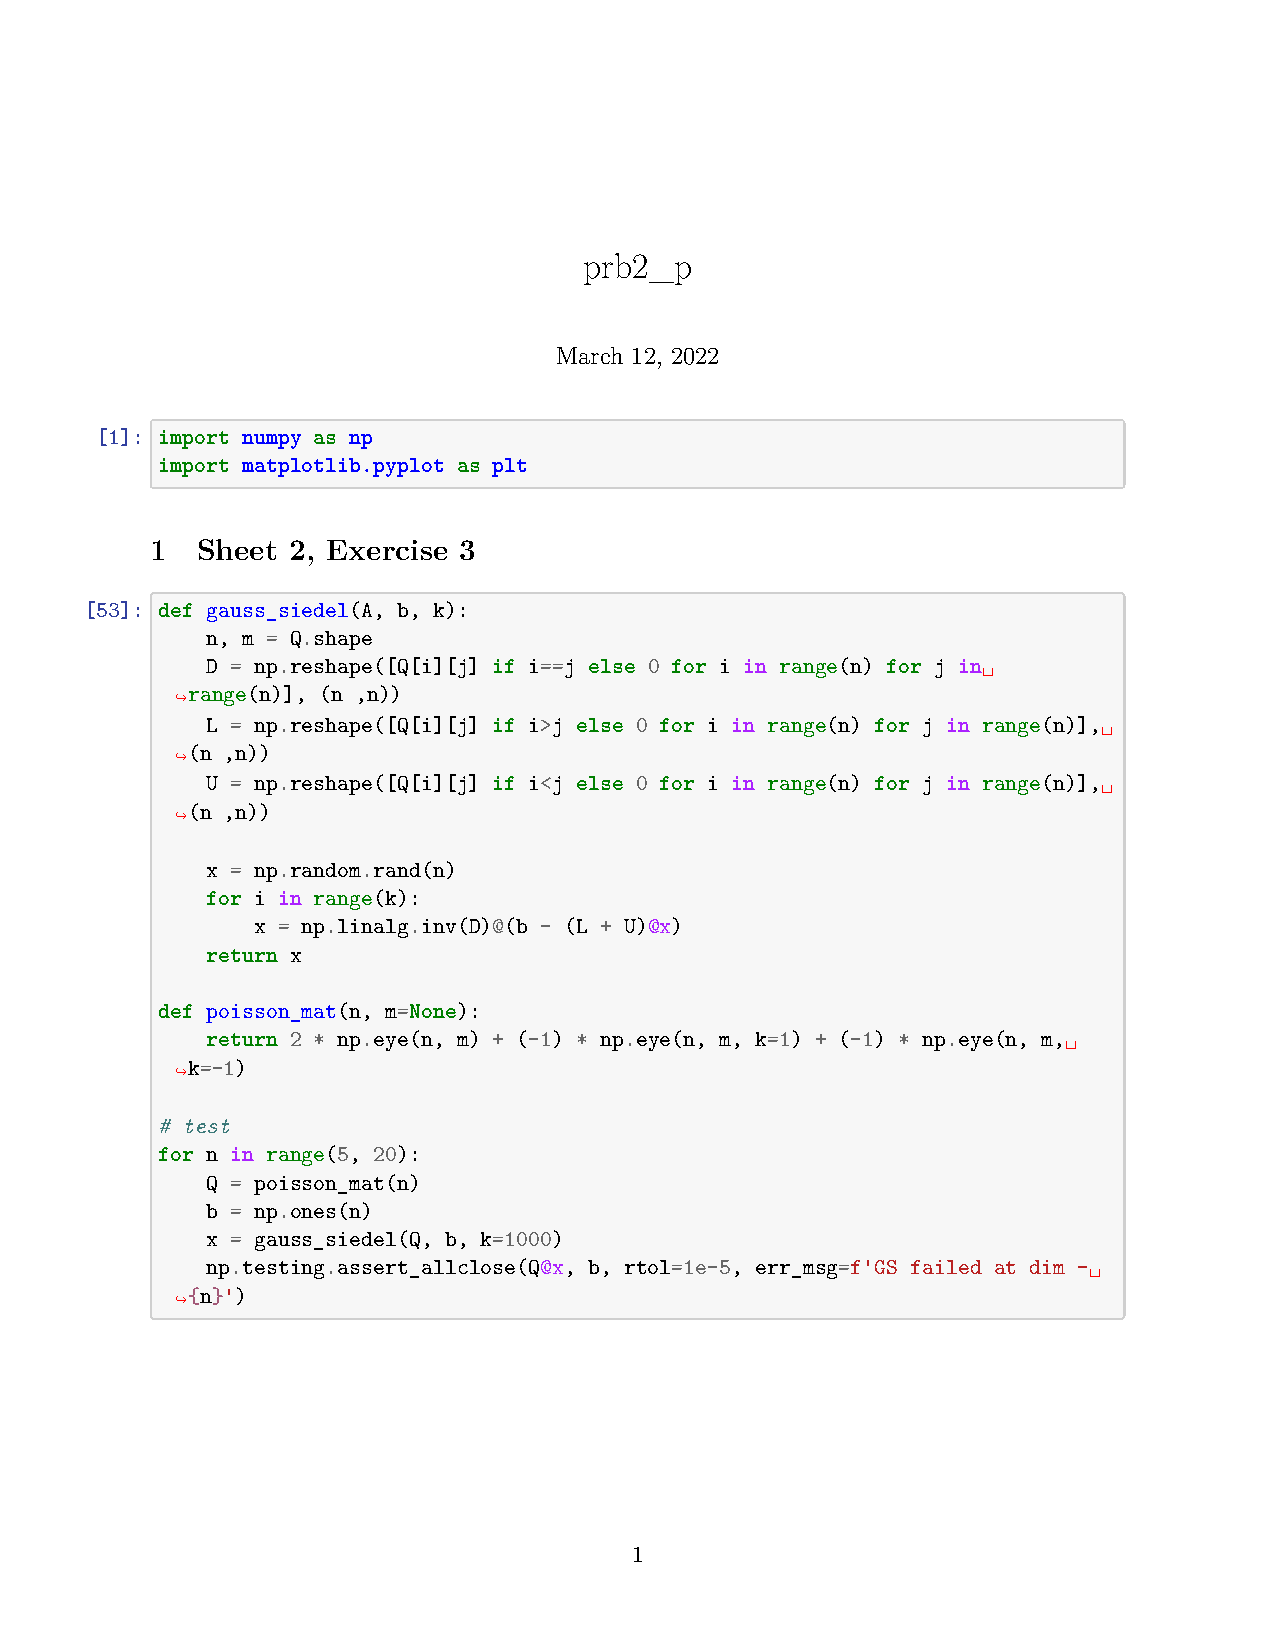
\includegraphics[width=0.8\textwidth, clip, trim=0cm 5cm 0cm 10cm]{./prog/prb2_p.pdf}
\end{figure}
\subsection{Problem 4}
Now let $P_n \in \mathbb{R}^{n\times n}$ be the matrix
\begin{align}
    P_n =
    \begin{pmatrix}
        2 & -1 &   &  & -1  \\
        -1& 2  & -1&  &   \\
          & \ddots  & \ddots & \ddots &   \\
          &   & -1 &  2 & -1\\
        -1 &   &  &  -1 & 2
    \end{pmatrix}
\end{align}
\subsubsection{}
(Can also be done with Gershorin disks)
\newline

We can show that all the eigenvalues of $P_n$ are in $[0, 4]$ because $P_n$
is the finite differenece/laplacian matrix for periodic boundary conditions
and can be diagonalized by a DFT. So let $\left( \lambda, v \right)$ be the
eigen-pair of $P_n$, which satisfy the equation
\begin{align}
    P_n v = \lambda v
\end{align}
This she standard Possion with periodic boundary conditions, with the
eigenvector $v_j = \omega^{jk} = e^{2\pi i \frac{jk}{n}}$ for a $j \in
\{1,\ldots,n\}$.
\begin{align}
    (P_n v)_j
    &= 2\omega^{jk}- \omega^{(j-1)k} - \omega^{(j+1)k}\\
    &= \omega^{jk}(2 - \omega^{-k} - \omega^{k})\\
    &= \omega^{jk}(2 - 2\cos\left( \frac{2\pi k}{n} \right)\\
    &= 4\sin^2\left( \frac{2\pi k}{n} \right) \omega^{jk} = \lambda_k v^k_j,
\end{align}
thereby we can conclude that $\lambda_k \in [0, 4]$ forall $k$.
\subsubsection{}
Because $P_n$ is a real, symmetric, cercular matrix the orthogonal components
of the eigenvalues are also eigenvectors, i.e. $\text{Re}\left(v \right)$ and
$\text{Im}\left(v \right) $. We may conclude this by pure calculation. In the $j-th$
component we have $k$ eigenvalues
\begin{align}
    \left(P_n\text{Re}\left( v^k \right)\right) _j
    &= 2\text{Re}\left( \omega^{jk} \right) -\text{Re}\left( \omega^{(j-1)k}
    \right) -\text{Re}\left( \omega^{(j+1)k} \right)\\
    &= \omega^{jk} +\omega^{-jk} - \frac{1}{2}\omega^{(j-1)k}
    -\frac{1}{2}\omega^{-(j-1)k}
    -\frac{1}{2}\omega^{(j+1)k} -\frac{1}{2}\omega^{-(j+1)k}\\
    &= \left( \omega^{jk} + \omega^{-jk} \right)
    -\frac{1}{2}\left( \omega^{jk}\left(\omega^{k} + \omega^{-k} \right)
    +\omega^{-jk}\left(\omega^{k} + \omega^{-k} \right)  \right)\\
    &= \frac{1}{2}\left( \omega^{jk} + \omega^{-jk} \right)\left(
    2-(\omega^{k} + \omega^{-k}\right) \\
    &= \text{Re}\left(\omega^{jk}  \right) \left(2-2\cos\left( \frac{2\pi
    k}{n}\right)\right)\\
    &= 4\sin^2\left( 2\pi \frac{k}{n} \right) \text{Re}\left( \omega^{jk}
    \right)  = \lambda_k\text{Re}(v^k_j).
\end{align}
\subsubsection{}
We define the quantity $m(n) = \min\{|\lambda|:\lambda\; \text{eigenvalue of
$P_n$}\}$. We can show that the quantity converges to 0 as $n$ goes to
infinity by calculating for a $k$ that minimises $\lambda_k$ which is for a
$k\neq$.
\begin{align}
    \lim_{n \to \infty}m(n)
    &= \lim_{n \to \infty}\min_{k\in\{1,\ldots,n\}}\{|\lambda_k(n)|\} = \lim_{n
    \to \infty}4\sin^2\left(2\pi \frac{k}{n}\right)\\
    &= \lim_{n \to \infty}4\cdot\left(\frac{x^2}{n^{2}} + \frac{x^{4}}{n^{4}}
    + O(\frac{1}{n^{6}})\right) = 0,
\end{align}
where $x = 2\pi k$.
\subsection{Problem 5}
Let $Q$ be like in Problem 3. And split $Q$ as
\begin{align}
    Q = D-N,
\end{align}
where $D$ consists of diagonal entries of $Q$. For $p \in \mathbb{N}$ let $C_p$ be the
Neumann polynomial preconditioner , defined as
\begin{align}
    C_p = D^{-1}\sum_{k=0}^{p} \left( ND^{-1} \right)^{k}
\end{align}
\subsubsection{}
\subsubsection{}
The following is a Phython script, that takes $n, p$ as an Input and returns
$C_p$ furthermore calculates the spectral condition number of the matrix
$C_pQ$
\begin{figure}[htpb]
    \centering
    \includegraphics[page=2 ,width=\textwidth, clip=true, trim=0cm 7cm 0cm
    3cm]{./prog/prb2_p.pdf}
    \includegraphics[page=3 ,width=0.8\textwidth, clip=true, trim=0cm 17cm 0cm
    2.5cm]{./prog/prb2_p.pdf}
\end{figure}
%\printbibliography
\end{document}

